% Created 2017-02-12 Sun 15:49
\documentclass[presentation]{beamer}
\usepackage[utf8]{inputenc}
\usepackage[T1]{fontenc}
\usepackage{fixltx2e}
\usepackage{graphicx}
\usepackage{longtable}
\usepackage{float}
\usepackage{wrapfig}
\usepackage{rotating}
\usepackage[normalem]{ulem}
\usepackage{amsmath}
\usepackage{textcomp}
\usepackage{marvosym}
\usepackage{wasysym}
\usepackage{amssymb}
\usepackage{hyperref}
\tolerance=1000
\usepackage{lmodern}
\usepackage{mathtools}
\usepackage{url}
\usepackage{color}
\usepackage{amssymb}
\usepackage{amsopn}
\usepackage{nicefrac}
\usepackage{units}
\usepackage{gensymb}
\institute[CERN, CLASSE, CINVESTAV]{\inst{1} Organisation Européenne pour la Recherche Nucléaire \and \inst{2} University}
\AtBeginSection[]{\begin{frame}<beamer>\frametitle{Content}\tableofcontents[currentsection]\end{frame}}
\institute[CERN, CLASSE, CINVESTAV]{\inst{1} Organisation Européenne pour la Recherche Nucléaire \and \inst{2} University}
\title[IDP Movement]{Forecasting for IDP reception after disasters}
\author[Bosne, Groen, Guillermo]{\underline{Eric Bosne}\inst{1} Derek Groen\inst{2} Gerardo Guillermo \inst{1}}
\date{\today}
\setbeamerfont{navigation symbols}{size=\footnotesize}
\setbeamerfont{date}{size=\footnotesize}
\setbeamerfont{author}{size=\footnotesize,series=\bfseries,parent=structure}
\setbeamerfont{institute}{size=\tiny,series=\bfseries,parent=structure}
\usepackage{appendixnumberbeamer}
\addtocounter{framenumber}{-1}
\setbeamertemplate{navigation symbols}{\usebeamercolor[bg]{footline}\insertframenumber/\inserttotalframenumber}
\author[Bosne, Groen, Guillermo]{\underline{Eric Bosne}\inst{1} Derek Groen\inst{2} Gerardo Guillermo \inst{1}}
\usetheme{Bergen}
\usefonttheme{}
\useinnertheme{}
\useoutertheme{}
\author{\underline{Eric Bosne}\inst{1} Derek Groen\inst{2} Gerardo Guillermo \inst{1}}
\date{\today}
\title{Forecasting for IDP reception after disaster}
\hypersetup{
  pdfkeywords={},
  pdfsubject={},
  pdfcreator={Emacs 25.1.1 (Org mode 8.2.10)}}
\begin{document}

\maketitle
\begin{frame}{Outline}
\tableofcontents
\end{frame}

\begin{frame}[label=sec-1]{Hackathon}
\begin{block}{O}
Identified some factors that might influence the movement of a person fleeing
from a conflict zone.
\end{block}
\begin{block}{O}
Built a simple decision making model with these factors and included it in
the flee library.
\end{block}
\begin{block}{O}
Imported data from the \href{http://iraqdtm.iom.int/Introduction.aspx}{DTM}
\end{block}
\begin{block}{O}
Started drafting a journal article
\end{block}
\begin{block}{O}
Successfully ran the simulation.
\end{block}
\end{frame}

\begin{frame}[label=sec-2]{Simulation output}
\begin{block}{*}
This is are the worse and best results.
\end{block}
\begin{block}{Graphs}
\begin{columns}
\begin{column}{0.4\textwidth}

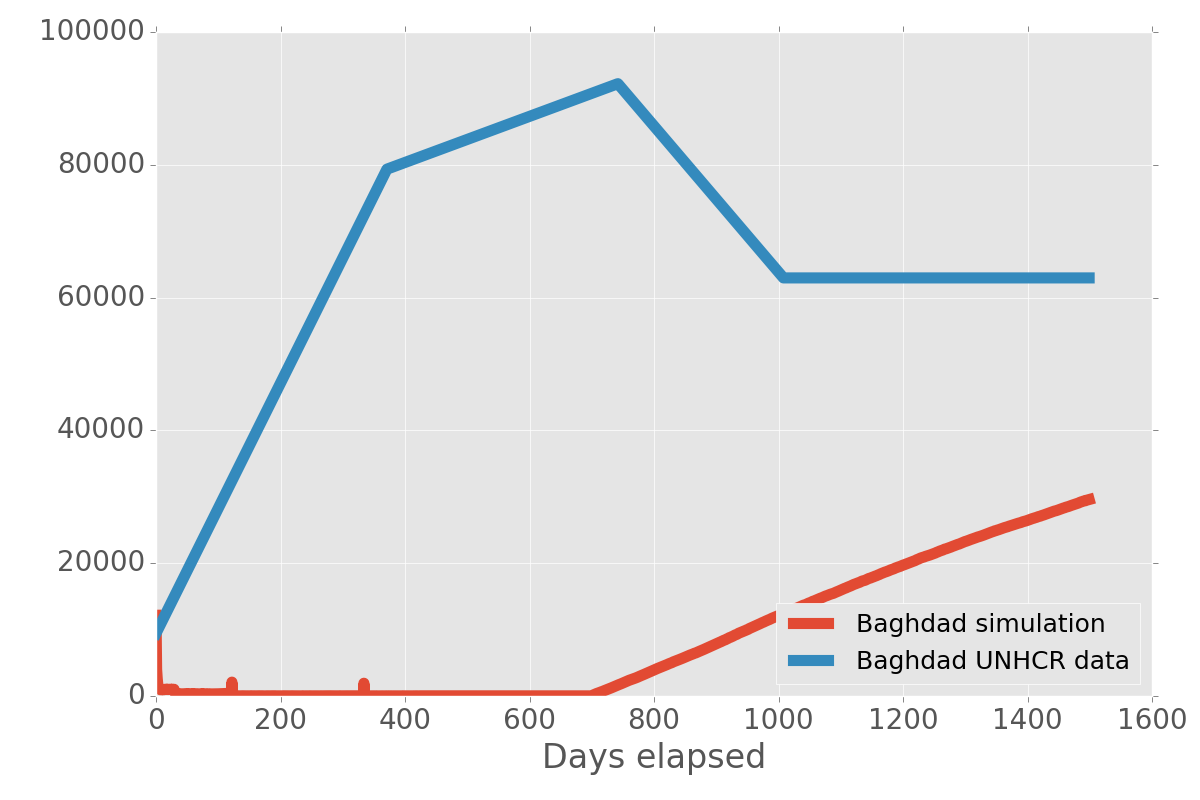
\includegraphics[width=.9\linewidth]{../../outiraq/Baghdad-4.png}
\end{column}
\begin{column}{0.4\textwidth}

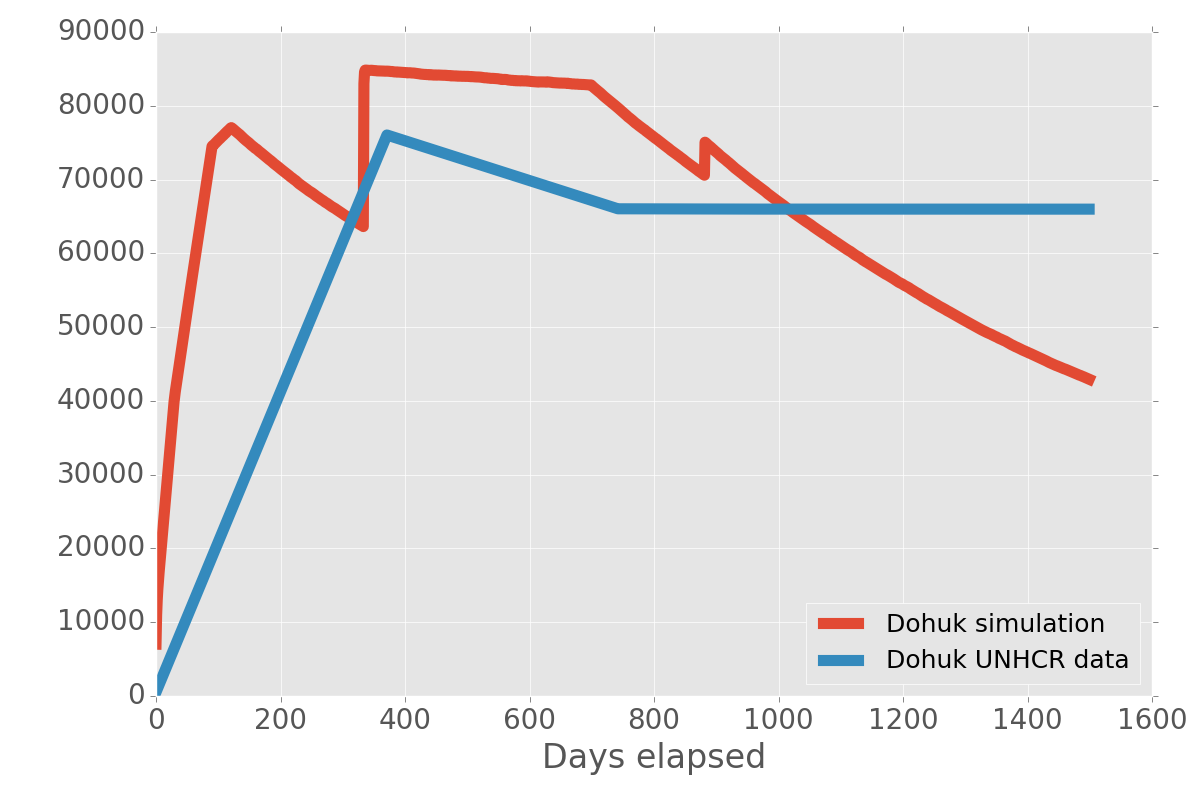
\includegraphics[width=.9\linewidth]{../../outiraq/Dohuk-4.png}
\end{column}
\end{columns}
\end{block}
\begin{block}{*}
What is important now is that we have a framework to study the effect of each
 factor.
\end{block}
\end{frame}
\begin{frame}[label=sec-3]{Post-Hackathon}
\begin{block}{O}
We all agreed we will continue the work aiming to publish it in a journal.
\begin{block}{-----}
\alert{Our to do list}
\end{block}
\begin{block}{O}
Optimize the model with the current factors.
\end{block}
\begin{block}{O}
Include left out parameters.
\end{block}
\begin{block}{O}
Automating the data imports.
\end{block}
\begin{block}{O}
Writting a final version.
\end{block}
\end{block}
\end{frame}
% Emacs 25.1.1 (Org mode 8.2.10)
\end{document}
